% 03-data-exploration-and-preprocessing-appendix.tex

\vspace{-0.5cm}

% Section Title
\section{DATA EXPLORATION AND PRE-PROCESSING}

    % Main Content

    This appendix contains additional plots and visualizations related to the data exploration and pre-processing phase of the analysis. The figures are grouped into subsections based on their thematic relevance.

    \subsection{Temporal Analysis of Attacks}

        % This subsection presents visualizations related to the temporal distribution of SSH attacks, including trends over hours, days, months, and years.

        \subsubsection{Attack Frequency by Hour \\}
        
            The plot shows the distribution of SSH attacks across different hours of the day. It reveals specific hours when attack activity peaks, which could indicate targeted times for malicious activities. Understanding these patterns can help in implementing time-based security measures.
            
            \vspace{-0.1cm}

            \begin{figure}[H]
                \centering
                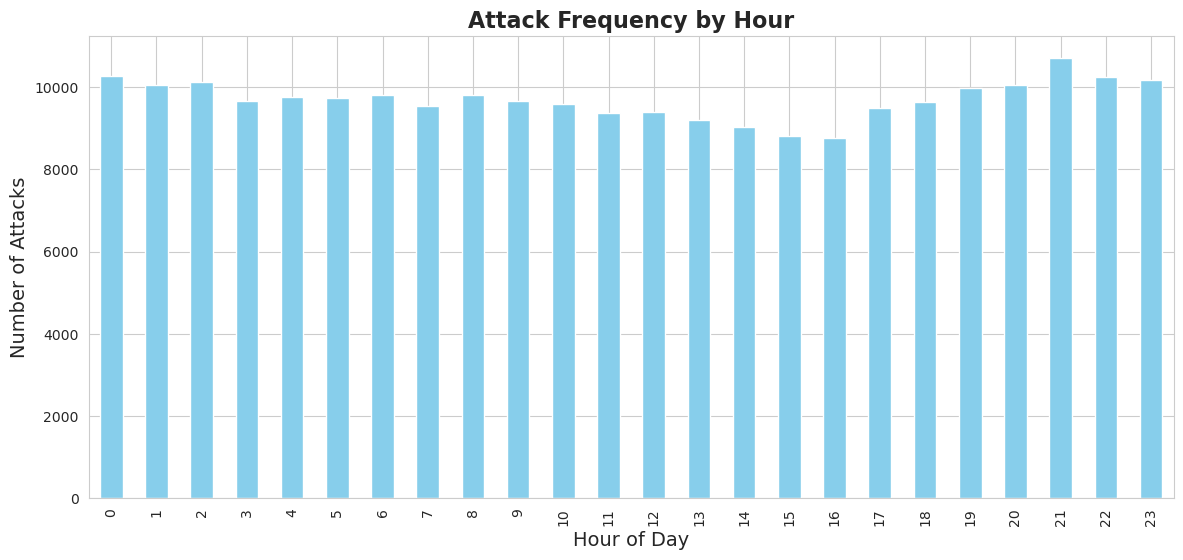
\includegraphics[width=0.7\textwidth]{../figures/plots/section1/attack_frequency_by_hour.png}
                \caption{Distribution of SSH attacks by hour of the day - The plot highlights peak hours during which attacks are most frequent}
                \label{fig:attack_frequency_by_hour}
            \end{figure}
        
        \clearpage % TODO: check
        
            The attacks are relatively well-distributed throughout the day, but notable peaks occur between 19:00 and 6:00, with lower activity observed from 9:00 to 16:00. This pattern might be explained by the likelihood that attackers schedule their activities during non-working hours when individuals and organizations are less likely to monitor or respond to security incidents.

        \subsubsection{Attack Frequency by Month \\}
        
            This plot illustrates the distribution of SSH attacks across different months. It highlights seasonal trends, showing months with higher attack frequencies. Such insights can be useful for anticipating periods of increased security threats and allocating resources accordingly.

            \vspace{-0.1cm}

            \begin{figure}[H]
                \centering
                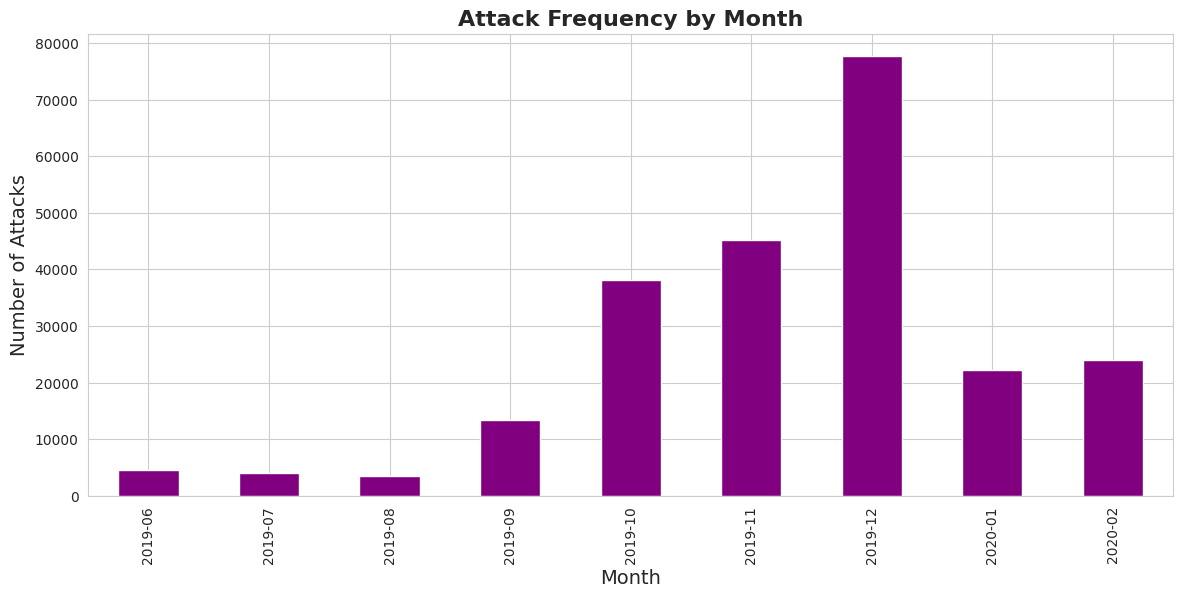
\includegraphics[width=0.68\textwidth]{../figures/plots/section1/attack_frequency_by_month.png}
                \caption{Distribution of SSH attacks by month - The plot reveals seasonal trends in attack frequency}
                \label{fig:attack_frequency_by_month}
            \end{figure}
            
            \vspace{-0.1cm}
            
            The number of attacks shows a noticeable increase from October to December, followed by a return to lower and more constant levels in the subsequent months. This trend raises the question of whether a seasonal pattern exists, possibly linked to factors such as end-of-year activities, holidays, or specific campaigns by attackers during this period.

        \subsubsection{Attack Frequency by Year \\}
        
            The plot compares the frequency of SSH attacks between the years 2019 and 2020.
            
            \vspace{-0.05cm}

            \begin{figure}[H]
                \centering
                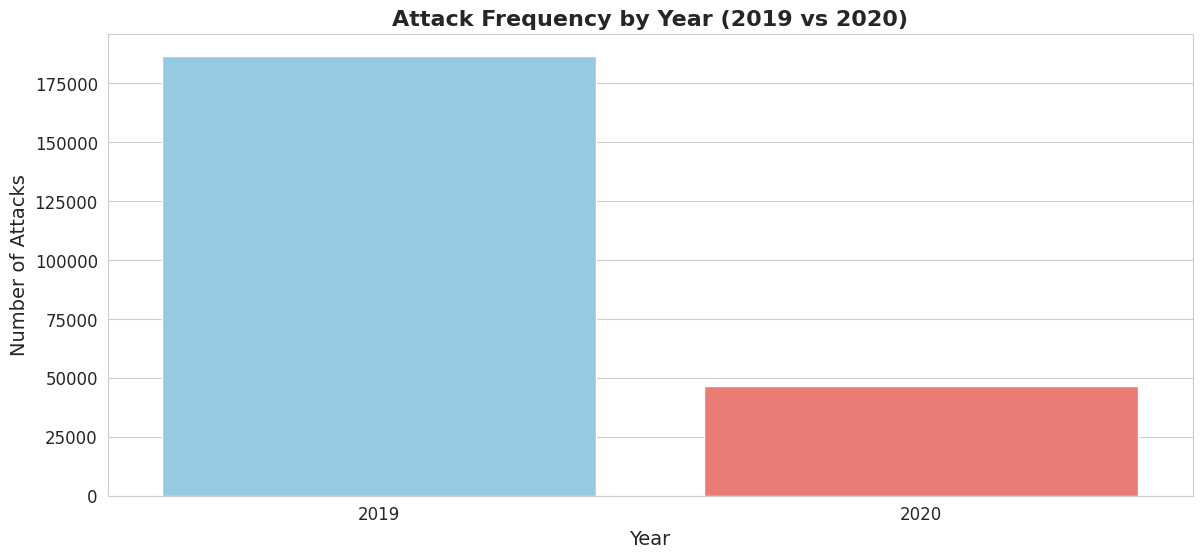
\includegraphics[width=0.68\textwidth]{../figures/plots/section1/attack_frequency_by_year.png}
                \caption{Distribution of SSH attacks by year - The plot shows the overall trend of attacks over multiple years}
                \label{fig:attack_frequency_by_year}
            \end{figure}
            
        \subsubsection{Temporal Series of SSH Attacks \\}
        
            This time series plot illustrates the distribution of SSH attacks over time, providing a clear view of how attack frequency fluctuates throughout the dataset. When combined with other plots, such as those highlighting daily or seasonal patterns, it enables a more comprehensive temporal analysis, helping to uncover deeper insights into attack trends and dynamics.

            \begin{figure}[H]
                \centering
                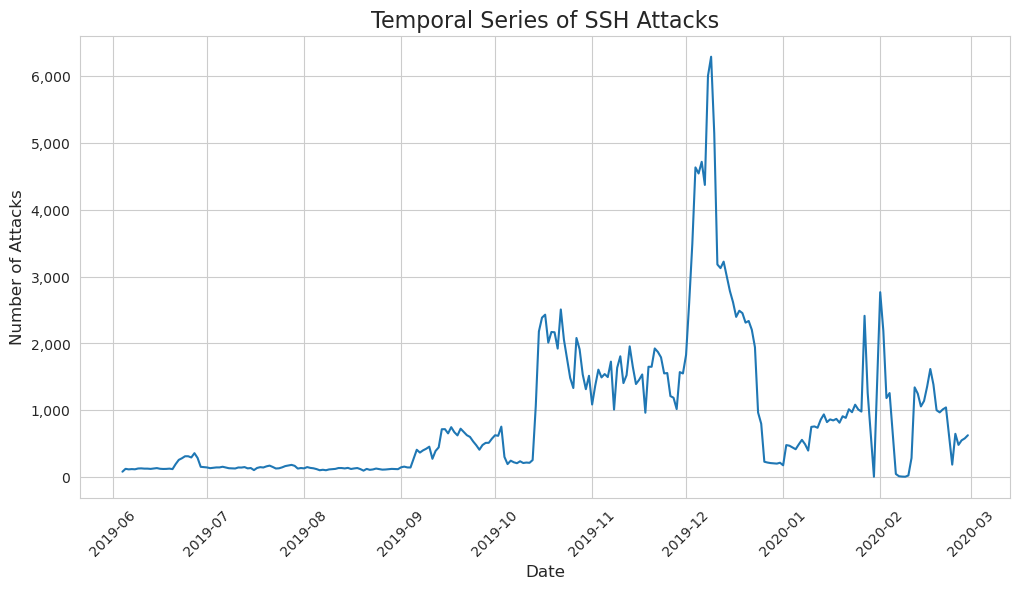
\includegraphics[width=0.7\textwidth]{../figures/plots/section1/temporal_series_of_ssh_attacks.png}
                \caption{Time series plot of SSH attacks over the entire dataset - The plot provides a view of attack patterns over time}
                \label{fig:temporal_series_of_ssh_attacks}
            \end{figure}

        \subsubsection{Intents Over Timestamps \\}
        
            The plot visualizes the distribution of different attack intents over time. It categorizes the intents: Defense Evasion, Harmless, Impact, Discovery, Persistence, Execution, and Others. By analyzing this plot, we can identify which intents are more prevalent at specific times, helping to prioritize security measures based on the nature of the threats.

            \begin{figure}[H]
                \centering
                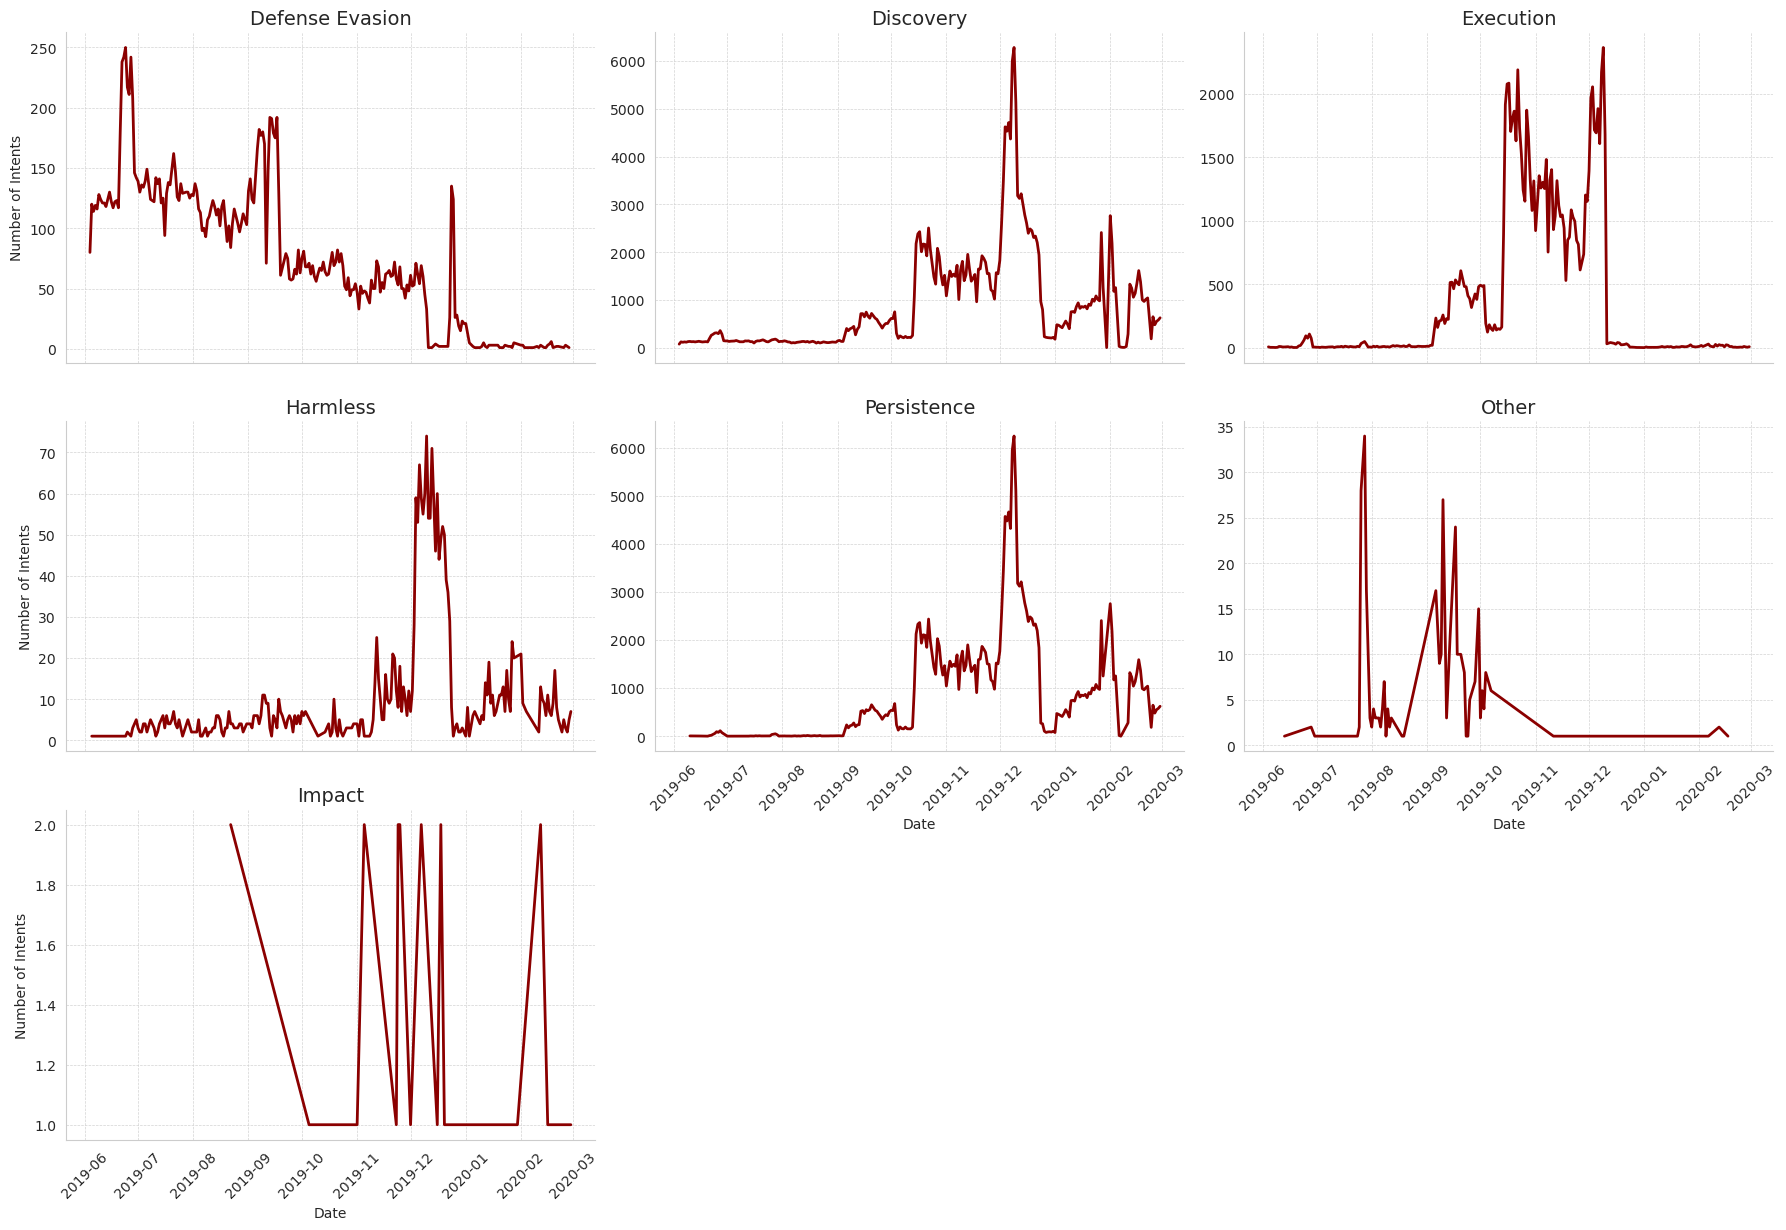
\includegraphics[width=0.9\textwidth]{../figures/plots/section1/intents_over_timestamps.png}
                \caption{Attack intents over timestamps - The plot provides insights into the temporal patterns of different attack intents}
                \label{fig:intents_over_timestamps}
            \end{figure}
            
    \clearpage % TODO: check
